\section{Branch-and-Bound Optimization}

%\begin{itemize}
%\item Describe the motivation to use the branch-and-bound to approach the efficiency issues (execute all queries are costly)
%\item The idea is to execute the minimum amount of queries.
%\item Describe the heuristic used to determined when evaluate a query
%\item Describe how those heuristic are used in the framework
%\item Describe how we tackle the time issue.  (reordering queries).
%\item Describe the moment  that attribute queries are generated. (at the beginning of the process)
%\item Describe the moment the queries with class clauses are generated. (they are generated when the cardinality of candidates are above a threshold)
%\item Describe how the predictor can increase the efficiency by skipping queries
%\item Describe how we train the classifier. it is done automatically after it converges.
%\end{itemize}

Suppose you have the following source data represented as triples:
\begin{lstlisting}[basicstyle=\LSTfont]
<sider:12312> <label> "Morphine"
<sider:12312> <type> <sider:Drug>
<sider:43434> <title> "Eosinophilic Pneumonia"
<sider:43434> <type> <sider:Drug>
\end{lstlisting}
And target data: 
\begin{lstlisting}[basicstyle=\LSTfont]
<drugbank:DB00295> <drugname> "Morphine Sulphate"
<drugbank:DB00295> <synonym> "Morphine"
<drugbank:DB00295> <type> <drugbank:Drug>
<drugbank:DB00494> <drugname> "Eosinophilic Pneumonia"
<drugbank:DB00494> <type> <drugbank:Drug>
\end{lstlisting}

For this example, each source predicate in $U^{*s}_A$ =\{\verb+label+, \verb+title+\} match all predicates in $U^{*t}_A$ =\{\verb+name+ and \verb+synonym+\}; therefore, there are four possible predicate alignment that could be exploited to find the match between the source and target instances, namely: $U^{*st}_A$ =\{$\langle label,drugname \rangle$, $\langle label,synonym \rangle$,$\langle title,drugname \rangle$, $\langle title,synonym \rangle$\}. Those pairs in  $U^{*st}_A$ form four possible template queries, assuming  only one type query (e.g. OR). For example, for the instance \verb+sider:12312+, two queries are possible (because $\{ title\}$ is not predicates for this instance):
$\langle drugname,"Morphine", OR \rangle^A$, 
$\langle synonym,"Morphine", OR \rangle^A$.
 
As any search optimization space, this set of possible choices (queries) forms a tree-shaped search space where each node represents a query and each level of the tree represents an instance. Then, the decision to be taken, it is to select a best query at each level of the tree. Fig. \ref{fig:sspace} depicts this search space.

 \begin{figure} [h]
\vspace{-10pt}
\centering
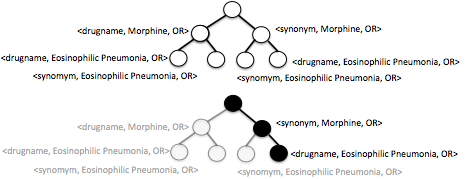
\includegraphics[scale=0.45]{p22.png}
\caption{The search space for an arbitrary example with 2 queries and 4 instances.} 
\vspace{-10pt}
\label{fig:sspace}
\end{figure}

Given $n$ source instances, $k$ different query types and $k$ comparable predicate pairs in $U^{*st}_A$, a naive approach would perform all $n \times k \times q$ queries to find the optimal candidate set for each instance. We show how this number of queries can be reduced through our branch-and-bound based optimization that aims to execute only a few effective queries for every source instance. 
 
\subsection{Search-based Optimization} 
The problem start by learning the schema alignments $U^{*st}_A$ from the data. Then , from this alignment, a initial set of template queries containing only attribute queries is created. Our initial search space is composed of $n \times k \times q$ queries. We conceive an iterative process where source instances are processed one by one, resulting in a tree-shaped search space where the tree nodes correspond to queries and each level of the tree represents an instance.  A path on this tree from the root to a leave indicates the queries selected for their respective instances. We will use node and query as synonyms from now on.

\subsubsection{Query Optimal Criteria} 

The goal of the optimization is to execute less queries as possible to determine the optimal one, as defined below:
\begin{definition}[Optimization Goal] Given a set of instances S and a set of template queries $Q =\{q_1,..., q_n\}$ and for every instance $s_i \in S$ exists a set of evaluated queries $Q^e_{s_i} \subset Q$, where $q^o_{s_i} \in Q^e_{s_i}$ is a optimal query for $s_i$, then the optimization goal is to minimize:
\[
{\arg \min} \bigcup_{s_i \in S}|Q^e_{s_i}| \land
{\arg \min} \bigcup_{s_i \in S} |q^o_{s_i}| 
\]
\end{definition} 

The optimal query for an instances can only be determined by evaluating all possible queries; however, to minimize the number of queries evaluated is one of the optimization goals. Both goals can be achieved simultaneously by making use of heuristics that helps to determined whether or not is necessary to evaluate a query.

Regarding the optimality of a query, the challenge is to select for each source instance the one fast query (few fast queries) needed to produce all and only the correct candidates. Thus, a query can be characterized by two dimensions, namely its \emph{execution time} and the \emph{optimality of its results}. As both criteria of optimality is not known, we propose a \emph{cardinality-based and time-based heuristics} that can estimate those criteria:

\begin{definition}[Cardinality Based Heuristic] The most optimal query is the one that yields exactly one candidate while queries with no results or too many results are less optimal. 
\end{definition} 
\begin{definition}[Time Efficiency Heuristic] A query is is optimal if it is time efficient.
\end{definition} 
The time efficiency heuristic captures the intuition queries that retrieves less elements are faster. While they are rather aggressive heuristics that are exclusively focused on reducing the number of candidates (not taking into account whether they are correct or not), we show it performs well in the experiments. 

Regarding the optimality of a the number of queries evaluated, not all queries need to be evaluate, because queries may produce subset of each other, intersecting candidate sets or even empty sets. For instance, suppose that the OR queries are superset of all other query types; consequently, a query OR cannot reduce the cardinality of a query AND, thus, it do not need to be evaluated if AND query retrieve a non-empty set. Complementary to this intuition, two queries that produces disjoint sets are both candidates to be optimal, because we cannot predict in which set are the correct matches (e.g. the query constructed from \verb+rdf:label+ retrieves candidates of type \verb+Ingredient+ while the query constructed from \verb+drugs:drugname+ retrieve \verb+Drugs+). These dependencies between template queries can be learned and used to skip the evaluation of subsequent queries.  Below we define an heuristic to capture this idea.

\begin{definition}[Candidates Intersection Heuristic] Given two distinct template queries $q_i$ and $q_j$, where $|q_i| > 0$ and $|q_j| > 0$,  if $q_i \cap q_j = \emptyset$, then their optimal candidate set is given by $q_i \cup q_j$, otherwise, the query that with smaller cardinality is optimal.
\end{definition}  

The process on which the optimization task takes place is described next.

\subsection{Best-First Search With Branch-and-Bound Pruning} 
 
Based on these heuristics, we use best-first search with branch-and-bound pruning~\cite{DBLP:journals/jacm/DechterP85} to execute only the best queries in the search space. The overall procedure is presented Alg.~1, which has three main components. It has a \emph{bounding policy}, which decides when to stop the whole process. The \emph{branching policy} determines the visit order of nodes within every level and when to move to a next level, based on cardinality and time estimates. Further, a classifier helps the branching policy to decide whether to skip certain queries or not. 

\textbf{Branching}. It is a breadth-first search procedure that processes queries associated with the source instance of the current level before moving to the next instance in the next level. In every level, this search is guided by the branching policy, which always selects the node that is best w.r.t.~ time and cardinality dimensions. More precisely, it chooses the one with lowest cardinality and among those not distinguishable in terms of that, it chooses the one that requires less time (based on the estimated values discussed before). 

According to the cardinality-based  this policy indicates to stop and to move to the next level when a node with cardinality 1 is visited (because there are no better queries than this).  However, according to the candidates intersection heuristic, an optimal candidate set is the union of non-empty and non-intersection optimal queries. We observed that non-intersecting queries occurs only for template queries build from different target predicates. Therefore, the cardinality-based is applied on set of template queries that share the same target predicate. For a N different target predicates, at least N queries are performed per instances. Once the optimal queries are found for each those sets, the search moves on to the next level. However, this process can be further optimized, by merging sets where their optimal queries produce intersecting results. To so, we apply a predictor that learns to predict from the history of queries processed in a previous levels, whether exist intersection optimal queries and which are those queries. 

\textbf{Query Predictor}. 
The predictor uses the candidate intersection heuristic to decide if a query should be evaluated or not. To exploit this, we train a classifier, which given a sequence of queries, predicts if the current node has lower cardinality than any other previous queries. Beside of that, it also predicts, if the results of current query does not intersect with the result of any other previous query. Therefore, the current query are evaluated only if any of these two conditions are satisfied.  While the branching policy can help to find optimal candidate sets, the predictor help to reduce the number of queries evaluated per level; in this way, we achieve the optimization goal.

\textbf{Bounding}. While the branching policy determines the next node to evaluate (and to stop processing one level when the optimal query is found)  the \emph{bounding policy} decides when to stop the whole process. The search should terminate when there exist no or too few matches for the source instances. This can be decided when through many levels, empty candidates sets are obtained as results. As shown in Alg.~1, the bounding strategy is 
controlled by the parameter $\gamma$. In the experiments in this paper, early termination through bounding is not used because we know in advance that matches exist between the datasets. 
\begin{algorithm}
\caption{CandidateSelection(G, G'). Find candidates for instances in $G$.}
\begin{algorithmic}
\scriptsize\tt
\STATE  sourcekeys  $\leftarrow$ FindCandidateSchema(G)
\STATE  targetkey  $\leftarrow$ FindCandidateSchema(G')
\STATE  keypairs  $\leftarrow$ AligningSchemas(sourcekeys, G, targekeys, G') 
\STATE  nodes  $\leftarrow$ BuildNodes(keypairs) 
\STATE  learning  $\leftarrow$ true
\FORALL{b in targetkeys} % Builds a classfier per target key
\STATE predictor[b] $\leftarrow$ NayveBayesClassifier.new()
\ENDFOR 
\FORALL{i in $G$} % Find candidates for each source instance
\IF { $i \geq\gamma$ and candidates = $ \emptyset $ }  %  Validate the bounding policy
\STATE  return null //Satisfied bounding policy
\ENDIF
\FORALL{node in nodes}  
\STATE  b $\leftarrow$ node.targetkey
\IF {cost[b] = 1}  
\STATE next //Satisfied branching policy 
\ENDIF
\IF {learning or predictor[b].predict(node)}  
\STATE  cost[b] = node.evaluate(i) 
\STATE  processed[b] $\leftarrow$  processsed[b] + node 
\IF {learning}  
\STATE    predictor[b].AddExample(node) //Learning Phase
\ENDIF 
\ENDIF 
\ENDFOR
\IF {$i \leq  \beta$} 
\STATE    SortNodesByElapseTime(nodes)  //Sort nodes 
\ENDIF
\IF {test error converges} 
\STATE    learning $\leftarrow$ false
\ENDIF
\IF {$i =ß \alpha$} 
\STATE  examples  $\leftarrow$ matcher(candidates)
\STATE  nodes  $\leftarrow$ updateNodes(examples) 
\STATE    learning $\leftarrow$ true
\ENDIF
\STATE  candidates[i] $\leftarrow$ AggregateMinimalCandidatesSet(processed)
\ENDFOR 
\RETURN candidates[i]
\end{algorithmic}
\end{algorithm}

\subsection{Leaning to Predict Query Optimality} 
Preceding the \emph{Learning} Phase in the Alg. 1, we describe a \emph{Sorting}  phase, aiming to process the queries that are time efficient first. Basically, nodes are sorted by their average evaluation time. Average time and this order are computed after $\beta \%$ of the instances have been processed. This order is kept to train the predictor and also used during the Prediction phase (so that branching continues with the query that requires lesser time, given they all equal in terms of cardinality). The $\beta$ parameter can be set to be small to obtain average time simply after a few instances (we set it to $1\%$ in the experiment).
 
In the \emph{Learning} phase, the predictor is learned as a Naive Bayes classifier~\cite{Hand2001Idiots}.  It predicts whether the current node to be chosen by the branching strategy indeed has lower cardinality or do not intersect with preceding nodes results . As features, we use the  identifier of a current query and a boolean value indicating if any previous query has cardinality greater than zero (i.e. whether it was executed before). 
Recall that the branching policy applies to queries constructed for every target predicate and it moves on to next queries when it found an optimal one. Similar to that, a predictor is learned for every set of nodes that share the same target predicate and accordingly, is only used for queries that have been constructed from this target predicate. The Learning phase stops soon after three iterations have the same test error. 
When the Learning phase terminates, both the branching policy and the predictor are applied to choose and to skip query nodes, respectively.  

In the \emph{Updating} phase, new template queries are generated with a class clause. The class queries are computed after $\alpha\%$ of the instances have been processed. In this work, we fix $\alpha$ to 5\% of the instances. Then, the candidates obtained so far are input to a matcher that outputs positive and negative examples. As a matcher,  the class-based disambiguator \cite{•} is used in this work. Those generated examples are input to the algorithm that computes the class clauses. For each class clause found a new query is created by adding it to the original queries. For $q$ queries and $n$ class clauses, then $n \times q$ new queries are generated in the end. After this process, the classifier is retrained using the Leaning procedure described before. 

 